\documentclass[tikz,border=10pt]{standalone}
\usepackage[T1]{fontenc}
\usepackage{lmodern}
\usetikzlibrary{arrows.meta,shapes.geometric}
\begin{document}
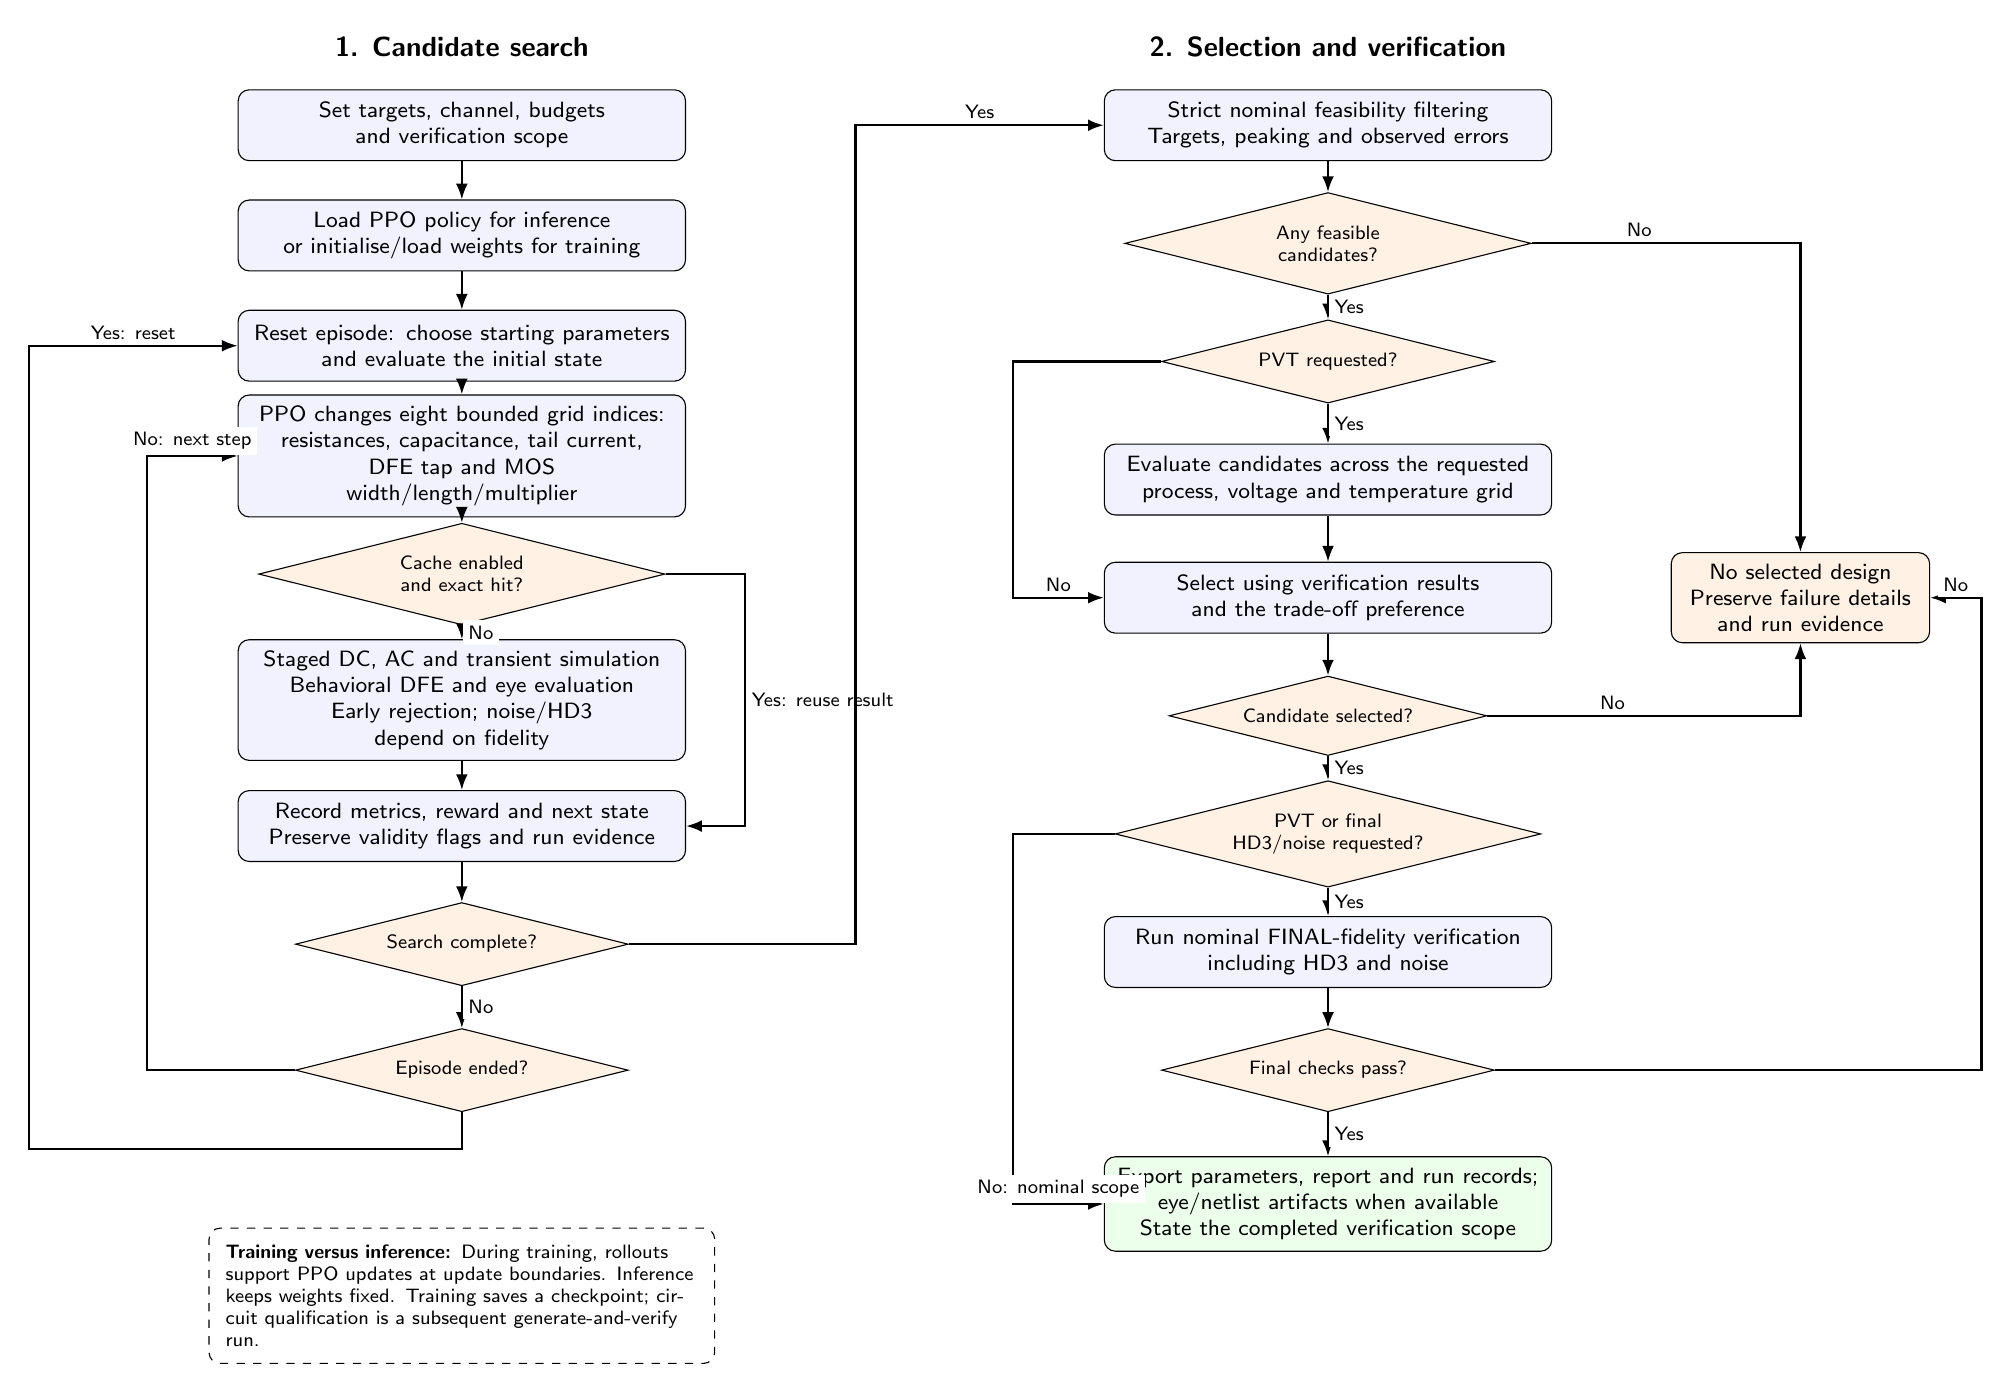
\begin{tikzpicture}[
font=\sffamily\footnotesize,
flow/.style={-{Latex[length=2mm]},thick},
box/.style={draw,rounded corners,fill=blue!5,text width=5.4cm,align=center,minimum height=9mm,inner sep=4pt},
decision/.style={diamond,aspect=4,draw,fill=orange!10,text width=3cm,align=center,inner sep=1pt,font=\sffamily\scriptsize},
edgeLabel/.style={font=\sffamily\scriptsize,fill=white,inner sep=2pt}
]
\node[font=\sffamily\bfseries] at (0,1) {1. Candidate search};
\node[font=\sffamily\bfseries] at (11,1) {2. Selection and verification};
\node[box] (input) at (0,0) {Set targets, channel, budgets\\and verification scope};
\node[box] (policy) at (0,-1.4) {Load PPO policy for inference\\or initialise/load weights for training};
\node[box] (reset) at (0,-2.8) {Reset episode: choose starting parameters\\and evaluate the initial state};
\node[box] (action) at (0,-4.2) {PPO changes eight bounded grid indices:\\resistances, capacitance, tail current,\\DFE tap and MOS width/length/multiplier};
\node[decision] (cache) at (0,-5.7) {Cache enabled\\and exact hit?};
\node[box] (evaluate) at (0,-7.3) {Staged DC, AC and transient simulation\\Behavioral DFE and eye evaluation\\Early rejection; noise/HD3 depend on fidelity};
\node[box] (feedback) at (0,-8.9) {Record metrics, reward and next state\\Preserve validity flags and run evidence};
\node[decision] (budget) at (0,-10.4) {Search complete?};
\node[decision] (episode) at (0,-12) {Episode ended?};
\node[box] (filter) at (11,0) {Strict nominal feasibility filtering\\Targets, peaking and observed errors};
\node[decision] (feasible) at (11,-1.5) {Any feasible\\candidates?};
\node[decision] (pvtrequest) at (11,-3) {PVT requested?};
\node[box] (pvt) at (11,-4.5) {Evaluate candidates across the requested\\process, voltage and temperature grid};
\node[box] (select) at (11,-6) {Select using verification results\\and the trade-off preference};
\node[decision] (selected) at (11,-7.5) {Candidate selected?};
\node[decision] (finalrequest) at (11,-9) {PVT or final\\HD3/noise requested?};
\node[box] (finalcheck) at (11,-10.5) {Run nominal FINAL-fidelity verification\\including HD3 and noise};
\node[decision] (accepted) at (11,-12) {Final checks pass?};
\node[box,fill=green!8] (output) at (11,-13.7) {Export parameters, report and run records;\\eye/netlist artifacts when available\\State the completed verification scope};
\node[box,fill=orange!10,text width=3cm] (failure) at (17,-6) {No selected design\\Preserve failure details\\and run evidence};

\foreach \a/\b in {input/policy,policy/reset,reset/action,action/cache,evaluate/feedback,feedback/budget,filter/feasible,pvt/select,select/selected,finalcheck/accepted}
 \draw[flow] (\a) -- (\b);
\draw[flow] (cache) -- node[edgeLabel,right]{No} (evaluate);
\draw[flow] (cache.east) -- (3.6,-5.7) -- node[edgeLabel,right]{Yes: reuse result} (3.6,-8.9) -- (feedback.east);
\draw[flow] (budget) -- node[edgeLabel,right]{No} (episode);
\draw[flow] (budget.east) -- (5,-10.4) -- (5,0) -- node[edgeLabel,above]{Yes} (filter.west);
\draw[flow] (episode.west) -- (-4,-12) -- (-4,-4.2) -- node[edgeLabel,above]{No: next step} (action.west);
\draw[flow] (episode.south) -- (0,-13) -- (-5.5,-13) -- (-5.5,-2.8) -- node[edgeLabel,above]{Yes: reset} (reset.west);
\draw[flow] (feasible) -- node[edgeLabel,right]{Yes} (pvtrequest);
\draw[flow] (feasible.east) -| node[edgeLabel,pos=0.2,above]{No} (failure.north);
\draw[flow] (pvtrequest) -- node[edgeLabel,right]{Yes} (pvt);
\draw[flow] (pvtrequest.west) -- (7,-3) -- (7,-6) -- node[edgeLabel,above]{No} (select.west);
\draw[flow] (selected) -- node[edgeLabel,right]{Yes} (finalrequest);
\draw[flow] (selected.east) -| node[edgeLabel,pos=0.2,above]{No} (failure.south);
\draw[flow] (finalrequest) -- node[edgeLabel,right]{Yes} (finalcheck);
\draw[flow] (finalrequest.west) -- (7,-9) -- (7,-13.7) -- node[edgeLabel,above]{No: nominal scope} (output.west);
\draw[flow] (accepted) -- node[edgeLabel,right]{Yes} (output);
\draw[flow] (accepted.east) -- (19.3,-12) -- (19.3,-6) -- node[edgeLabel,above]{No} (failure.east);

% Dedicated note area keeps annotations away from the diagram and return paths.
\node[draw,dashed,rounded corners,text width=6cm,align=left,
font=\sffamily\scriptsize,inner sep=6pt,anchor=north] at (0,-14)
{\textbf{Training versus inference:}
During training, rollouts support PPO updates at update boundaries.
Inference keeps weights fixed. Training saves a checkpoint;
circuit qualification is a subsequent generate-and-verify run.};
\end{tikzpicture}
\end{document}
